\documentclass[sigconf]{acmart}

\usepackage{algorithm}
\usepackage{algpseudocode}
\usepackage{amsmath}
\usepackage{placeins}
\usepackage{graphicx}
\usepackage{todonotes}



\AtBeginDocument{%
  \providecommand\BibTeX{{%
    \normalfont B\kern-0.5em{\scshape i\kern-0.25em b}\kern-0.8em\TeX}}}
\setcopyright{rightsretained}
\acmConference[SNACS '24]{Social Network Analysis for Computer Scientists Course 2024}{Master CS, Fall 2024}{Leiden, the Netherlands}
\copyrightyear{2024}
\acmYear{2024}
\acmISBN{}
\acmDOI{}
%%%% Do not modify lines 1-11

\begin{document}

\title{Hierarchical core-periphery structure in networks}
\subtitle{ Social Network Analysis for Computer Scientists --- Course paper} % do not modify this

\author{Davide Baggio}
%\orcid{0000-0001-5468-1030}
\email{d.baggio.2@umail.leidenuniv.nl}
\affiliation{
  \institution{LIACS, Leiden University (Erasmus+) \\ University of Padua}
  \city{}
  \country{}}

\author{Maksim Starostenko}
%\orcid{0000-0001-5468-1030}
\email{m.starostenko@umail.leidenuniv.nl}
\affiliation{
  \institution{LIACS, Leiden University}
  \city{}  
  \country{}}

\renewcommand{\shortauthors}{Baggio and Starostenko}

\keywords{hierarchical core-periphery,clustering, social network analysis, network science}

\begin{abstract}

% The abstract summarizes the entire paper: context, problem, solution, approach, data, concrete experimental results, conclusion and real-world implications. But, shortly, so in half a column or so. You may write this as the very last thing.

\end{abstract}

\maketitle

\section{Introduction}

% Textual description of the context, the main problem considered, why it is important, how it is addressed in other works (already providing some key references), and what real-world applications of this problem are. How is this paper going to contribute w.r.t. existing techniques and related/previous work? End with a (second-to-last) paragraph on what the contributions of the paper are (so, which problems you solve or which research questions you address), and finally a paragraph on how the remainder of the paper is organized.


%\item \textbf{Background:} Start with a brief introduction to core-periphery structures in networks, describing why they’re important in network science.
The core-periphery structure is a common type of clustering method used to detect underlying features in network graphs. Its main objective is to identify clusters in the network by extracting graph elements (nodes) based on their features and behavior. In this structure, core nodes are considered more central and important, while peripheral nodes are less important but still depend on the core nodes.

The core-periphery detection algorithm is essential for understanding the structure of various networks, offering valuable insights across a wide range of applications, from small-scale networks to large ones. It is particularly useful in analyzing and explaining relationships in diverse domains such as economic activity between countries or regions, as well as in social, biological, and financial networks.

The traditional core-periphery structure consists of two distinct groups: the core and the periphery. Nodes in the core are typically more densely interconnected together, while peripheral nodes have fewer connections between themselves and rely more heavily on the core nodes for connectivity. The connection between core and periphery can also be either highly concentrated or low-concentrated edge-wise. 
When the structure of a graph is extended to a multiple number of groups, the algorithm provides a flexible shift to a more complex structure of a network, where it accounts for all different kinds of possible structures of the network, meaning that there can be multiple cores, that are parallel, nested and located at different hierarchical levels of the network.

The following algorithm ensures a great generalization on a number of different possible structures, while other algorithms similar algorithms that try to identify core-periphery structure lack on capabilities of detecting special circumstances. For example k-core decomposition algorithm builds a structure based on the degree distribution of the nodes, which may not align well with an actual core-periphery structure. Other popular algorithms are "Quality Function" and "Stochastic Block Models". These algorithms are sensitive to the choice of parameters therefore they are very hard for optimization and prone to errors. 

While it might seem that the suggested algorithm is revolutionary and outstanding, i.e it's generalised and optimised to account for all variations of the structures. This fact still has to be double checked, therefore further experiments and testing are needed. The algorithm is to be tested on 15-20 \todo[inline]{15-20?} datasets in order to analyze and assess it's performance on various structures and settings. 



%The main advantage of the Hierarchical core-periphery algorithm over other algorithms is that it accounts for , while other 
%other algorithms tend to overlook some of the features that are accounted for by the given structure. 





 %   \item \textbf{Current Algorithm:} Summarize the hierarchical core-periphery detection algorithm, briefly explaining its purpose, functionality, and how it stands out compared to other approaches.
  %  \item \textbf{Research Gap:} Highlight the need for further analysis, especially regarding its performance across different types of networks. This shows the value of testing the algorithm on diverse datasets.
  %  \item \textbf{Objective:} Clearly state that your research aims to assess the algorithm’s effectiveness across 20 different datasets, specifying whether they span different domains, network structures, or scales.

\section{Related work}
% briefly discuss other papers related to this work, or previous work describing other approaches for the same problem. end with a statement on how your paper contributes to these works.
Over the years, researchers have explored various methodologies and perspectives on core-periphery structures, deepening our understanding of how these configurations influence network connectivity, robustness, and community organization.

One of the first studies to introduce core structures was the paper by Seidman \cite{seidman} in 1983, which proposed a method for identifying core nodes in social networks based on their connectivity, defining a k-core as a maximal subgraph where each node has at least k connections to other nodes within the subgraph. 
Subsequently, Borgatti and Everett \cite{borgatti} in 1999 formally introduced the core-periphery model, defining cores as densely connected nodes and peripheries as sparsely connected nodes linked primarily to the core. 

An important change was introduced by Rombach et al. \cite{rombach} in 2013, who proposed a method for detecting hierarchical core-periphery structures, allowing for the identification of multiple nested core layers within a single network. This approach provides a more nuanced understanding of network organization, enabling the analysis of multilevel interactions within complex networks.

A key reference for this study is the 2023 paper by Polanco and Newman, \textit{Hierarchical Core-Periphery Structure in Networks} \cite{hierarchical}. This work advances the understanding of core-periphery configurations by introducing a method for detecting nested core and periphery regions across multiple hierarchical levels, offering a richer perspective on the layered complexity within network structures. \\
Building on these foundational studies, our research aims to assess the effectiveness of hierarchical core-periphery detection across a diverse set of networks, contributing to the ongoing exploration of core-periphery structures in complex networks.

\section{Preliminaries}

% Necessary notation, formal definitions, if needed theorems, and a problem statement. Explain nontrivial notation upon first use. If applicable, give a formal problem statement and say something about space and time complexity. 
In this model, nodes are organized into overlapping groups, allowing for flexible membership across multiple categories. The rules for determining group membership and the probabilities of forming edges between nodes are described below. \\
\begin{itemize}
    \item Nodes can belong to any of the $k$ groups, which are labeled by $r = 0, ..., k - 1$ and all of them must also belong to group 0;
    \item The notation used to describe if a node belongs to a specific group is the following: $g_u^r = 1$ if node $u$ belongs to group $r$, and $0$ otherwise;
    \item We use a set of probabilities, $\omega_r$, for each group including group 0. Edges are placed between node pairs independently with probability $\omega_r$, where $r$ is the highest common group that both nodes in the pair belong to, meaning the one with the highest number. For example, if one node belongs to groups 0, 1, 2 and another belongs to 0, 1, 3, then there is an edge between them with probability $\omega_1$.
\end{itemize}
\vspace{0.3cm}
The end result is a graph that has the following characteristics:
\FloatBarrier
\begin{figure}[h]
    \centering
    \includegraphics[width=0.9\linewidth]{Img/cp general.png}
    \caption{General core-periphery structure.}
    \label{fig:general cp}
\end{figure}
\FloatBarrier
\todo[inline]{Montecarlo theorem?}


\section{Approach}
% Factually present your solution to the problem studied in the paper. This may include a repetition in your own words of the original paper that you studied. Strive to have at least one explanatory picture that explains the approach, perhaps using the tikz package, or more algorithmically using the algorithm(ic) package. Distinguish between previously introduced methods and your contribution clearly, for example by using subsections named after the various (components of the) approach(es).  

			
\section{Data} \label{sec:data}
% what datasets did you use, what types of networks do they represent, where did you obtain the data? did you do any processing? give a table describing data characteristics, such as number of nodes, edges, average degree, etc. 
% Is the data possible biased and how does this affect the experiments? 
As datasets, we use the following networks:
\begin{itemize}
    \item \textbf{Museum}: it's the directed network that represents the connections between rooms, which was created as part of Assignment 2 in the SNACS course.
    \begin{itemize}
        \item Nodes: 51;
        \item Edges: 70.
    \end{itemize}
    \item \textbf{Dolphins}: it's an undirected social network of frequent associations between 62 dolphins in a community living off Doubtful Sound, New Zealand. \cite{dolphins}
    \begin{itemize}
        \item Nodes: 62;
        \item Edges: 159.
    \end{itemize}
    \item \textbf{Karate}: it's an undirected social network of friendships between 34 members of a karate club at a US university in the 1970s. \cite{karate}
    \begin{itemize}
        \item Nodes: 34;
        \item Edges: 78.
    \end{itemize}
    \item \textbf{Les Miserables}: it's an undirected social network of characters in Victor Hugo's novel "Les Miserables". \cite{lesmiserables}
    \begin{itemize}
        \item Nodes: 77;
        \item Edges: 254.
    \end{itemize}
    \item \textbf{GoT}: it's the directed network of coappearances of characters in the Game of Thrones series, by George R. R. Martin. \cite{got}
    \begin{itemize}
        \item Nodes: 107;
        \item Edges: 352.
    \end{itemize}
\end{itemize}


\section{Experiments}
% Subsections on for example the experimental setup (which software, hardware and parameters did you choose), as well as the results of applying your approach to the data you described in preceding sections, leading to results that answer your research questions. You likely present some tables and figures. Remember captions and axis labels. 

% Think of incorporating the followng: What experiments can be used to compare, test and verify the suggested approaches? What do you measure in each experiment? Quality, running time, error size? Be precise. For datasets that perform either very well or not so well, try to find out why. Zoom in with additional experiments on noticeable results.  Can you relate the performance of the algorithms to some of the properties of the datasets? Or: can you define for which particular datasets a certain technique works well, and why? Make sure that the type of data/result that you want to communicate is suitable for the chosen presentation mode.
In this section we present the results of applying the hierarchical core-periphery detection algorithm to the datasets described in section \ref{sec:data}. 
\\We ran the algorithm on each network setting the parameter \\\verb|max_num_groups| to 5, which allows for the detection of up to 5 core-periphery groups in each network.
Please note that this means that the algorithm may detect fewer groups if the network does not contain enough structure to support the detection of 5 groups at the configuration with the smallest log-likelihood.
\FloatBarrier
\begin{figure}[h]
    \centering
    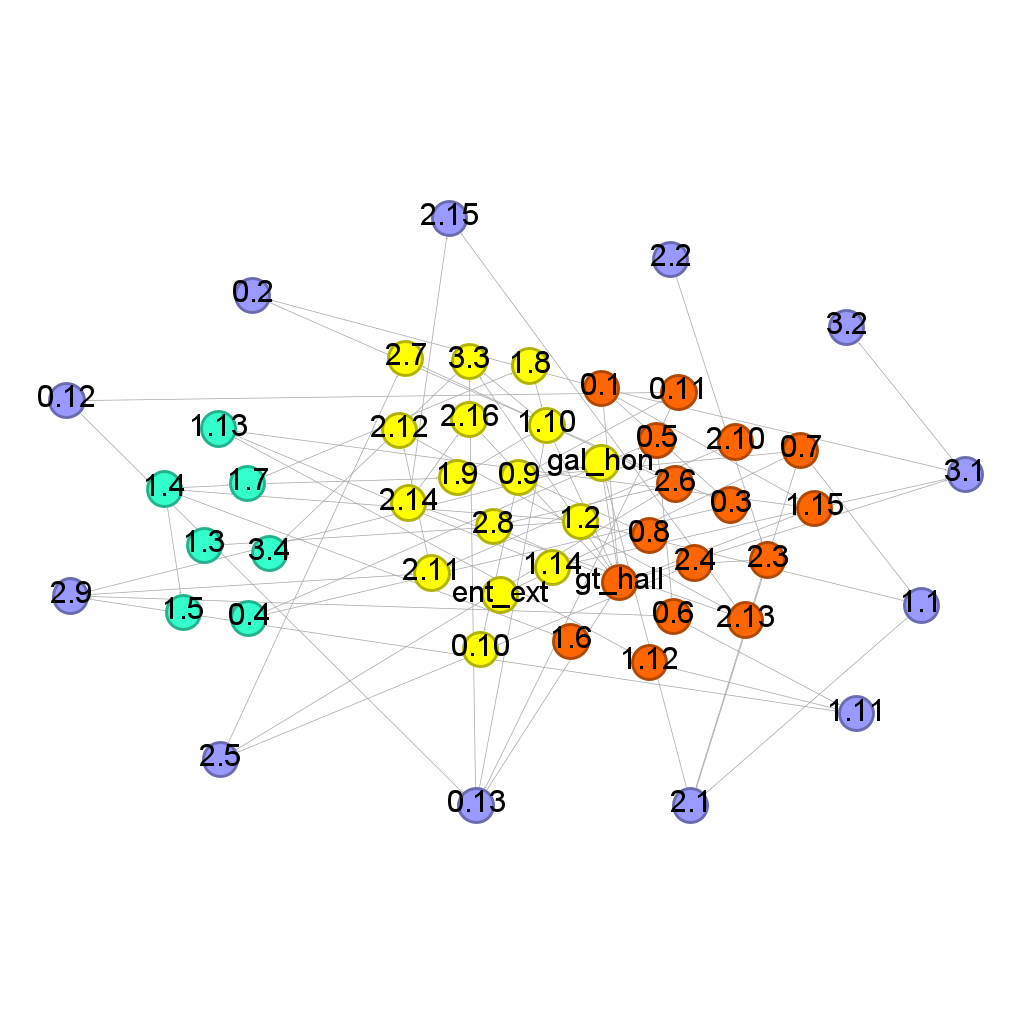
\includegraphics[width=\linewidth]{Img/museum 3 groups.png}
    \caption{CP museum dataset with 3 groups.}
    \label{fig:general cp}
\end{figure}
\FloatBarrier
\noindent In this graph we can observe that the algorithm detected 3 core-periphery groups in the museum network:
\begin{itemize}
    \item Group 0: lilac;
    \item Group 1: cyan;
    \item Group 2: orange/yellow.
\end{itemize}
The core-periphery structure is clearly visible, with the core nodes forming a dense cluster in the center of the network, while the peripheral nodes are located on the outskirts. The connections between the core and periphery are well defined, with the core nodes acting as bridges between the different groups.

\FloatBarrier
\begin{figure}[h]
    \centering
    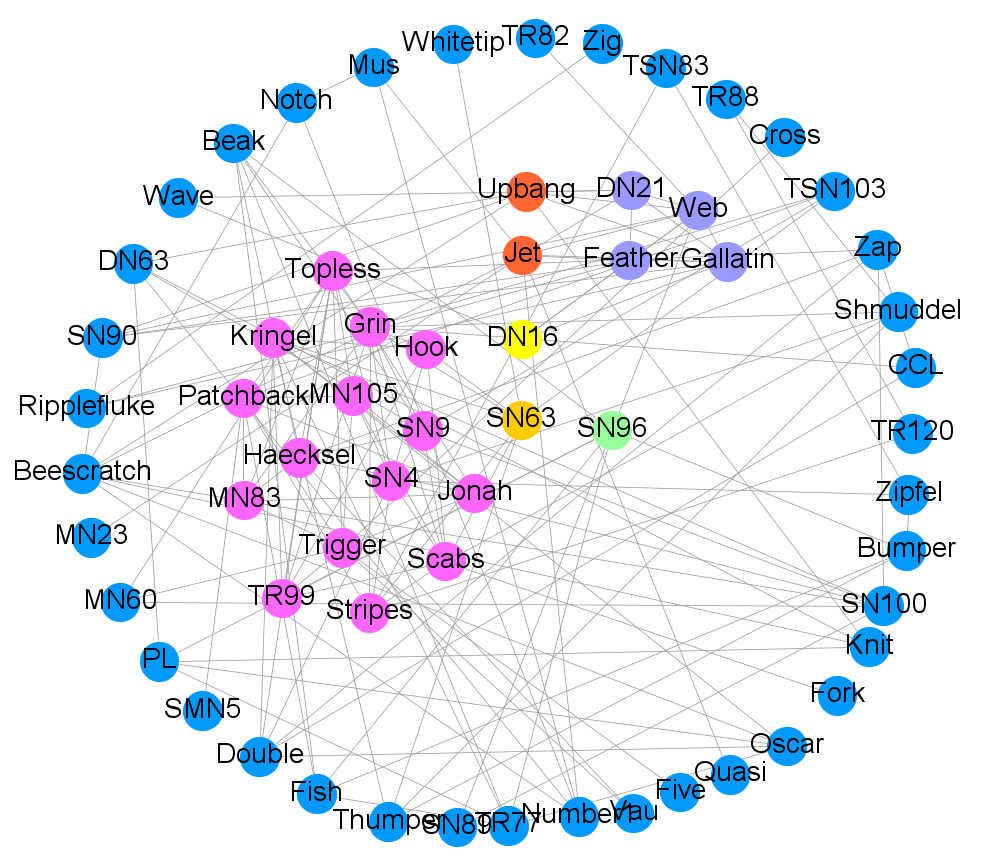
\includegraphics[width=1.05\linewidth]{Img/dolphins 4 groups.png}
    \caption{CP dolphins dataset with 4 groups.}
    \label{fig:general cp}
\end{figure}
\FloatBarrier
\noindent In this graph we can observe that the algorithm detected 4 core-periphery groups in the dolphin network:
\begin{itemize}
    \item Group 0: light-blue;
    \item Group 1: lilac/orange/yellow;
    \item Group 2: pink/ocher/yellow;
    \item Group 3: green/yellow/ocher/orange.
\end{itemize}
This graph representation is well-structured as well, but is slightly more complex to interpret. The added complexity arises from the presence of an additional group and the fact that many nodes belong to multiple groups.

\FloatBarrier
\begin{figure}[h]
    \centering
    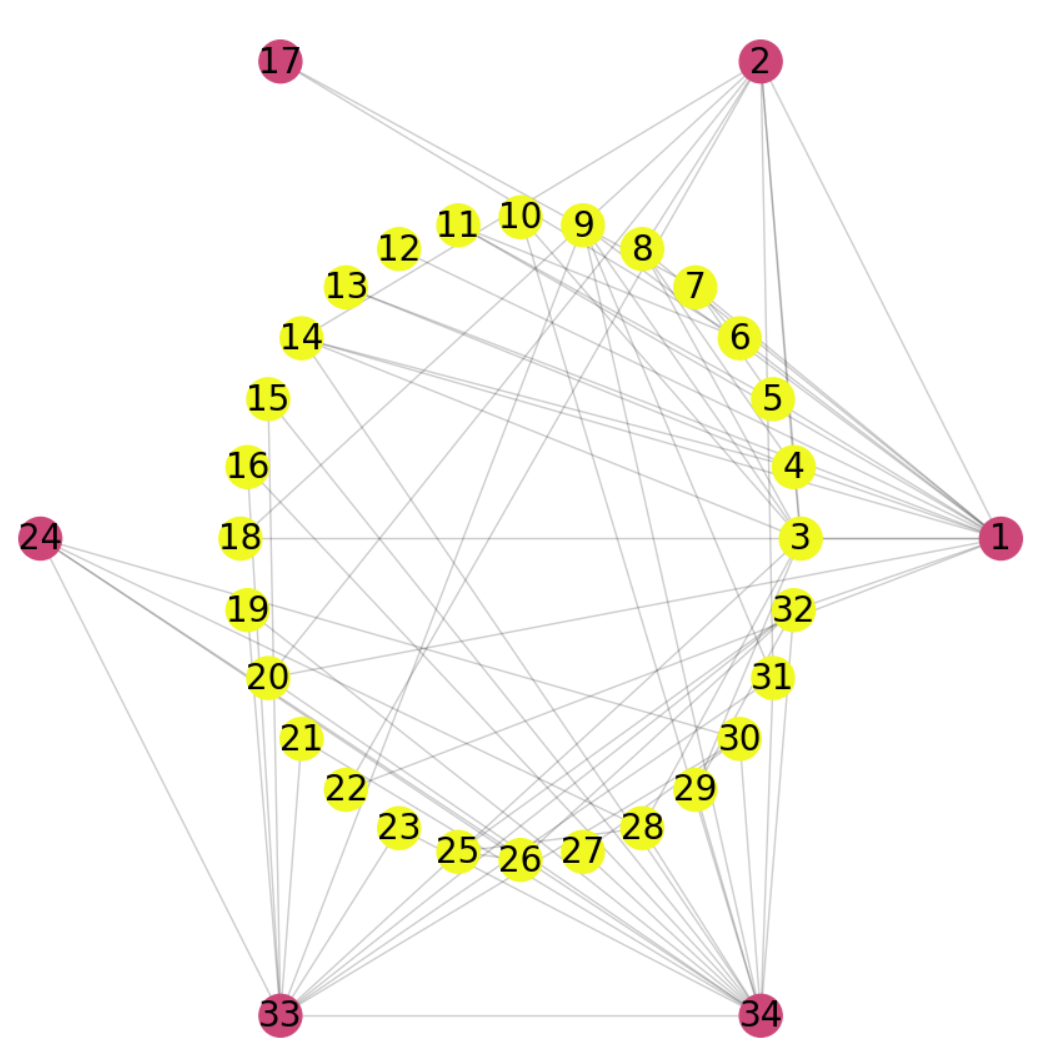
\includegraphics[width=\linewidth]{Img/karate 2 groups.png}
    \caption{CP karate dataset with 2 groups.}
    \label{fig:general cp}
\end{figure}
\FloatBarrier
\noindent This one is the first time that the algorithm detected the classic 2 core-periphery groups in the karate network:
\begin{itemize}
    \item Group 0: purple;
    \item Group 1: yellow.
\end{itemize}
The core-periphery structure is clearly visible, but we are not convinced that the algorithm separated the groups correctly. The peripheral nodes have many edges with the core nodes (in particular nodes 1 and 34), while many core nodes have few connections with other core nodes. This is a clear sign that the algorithm did not assign the nodes to the correct groups.

\todo[inline]{other datasets}

\section{Conclusion}

% summarize in at most one column the main results of the paper, stating how you addressed the problem statement and how the experiments help understand whether  the approach works (or not). end with one or two short suggestions for future work. 

% Think of the following: What was our problem statement again? (1 sentence) What was learned from the experiments? To what extend can the problem be solved? What works, what does not? What remain open problems? Can you give suggestions for future work in this area?

\begin{acks}
% optional: acknowledgments, so people or organizations you wish to thank 
\end{acks}

% You are responsibly for providing a list of complete and precise references. For an article (@article or @inproceedings), provide author, title of work, journal- or conference name, page numbers and year. For a book, provide author, title, press and year. For a website, provide author, title, URL and date accessed.

\bibliographystyle{ACM-Reference-Format}
\bibliography{snacspaper} % put your references in bibtex format in snacspaper.bib

%\appendix
%\section{Robustness checks}
% Appendixes are optional for the course project. they can contain proofs, figures or tables that do not fit in the main body of the text, but are handy as background information

\end{document}
\endinput
